\documentclass[11pt, openright, a4paper, brazil, openany, oneside]{abntex2}
\usepackage{lmodern}
\usepackage{verbatim}
\usepackage[T1]{fontenc}	
\usepackage[utf8]{inputenc}
\usepackage{times}	
\usepackage{indentfirst}	
\usepackage{color}			
\usepackage{graphicx}		
\usepackage{microtype} 		
\usepackage{multicol}
\usepackage{multirow}
\usepackage{lipsum}				
\usepackage[brazilian,hyperpageref]{backref}	 
\usepackage[alf]{abntex2cite}
\renewcommand{\backrefpagesname}{Citado na(s) página(s):~}
\renewcommand{\backref}{}
\renewcommand*{\backrefalt}[4]{
	\ifcase #1 %
		Nenhuma citação no texto.%
	\or
		Citado na página #2.%
	\else
		Citado #1 vezes nas páginas #2.%
	\fi}%
\titulo{Cálculo Numérico}
\autor{Sérgio Luís Soares Almeida \\ Matrícula 18/0006410}
\local{Brasília}
\data{2018, 02 de Outubro}
\instituicao{%
  Universidade de Brasília -- UnB
  \par
  Departamento de Matemática
  \par
 PROFMAT
  \par
  Professor José Eduardo Castilho}
\tipotrabalho{Relatório}

\definecolor{black}{RGB}{0.0,0.0,0.0}


\makeatletter
\hypersetup{pdftitle={\@title}, pdfauthor={\@author}, pdfsubject={\imprimirpreambulo}, pdfcreator={LaTeX with abnTeX2}, pdfkeywords={abnt}{latex}{abntex}{abntex2}{relatório técnico}, colorlinks=true, linkcolor=black, citecolor=black, filecolor=black, urlcolor=black, bookmarksdepth=4}
\makeatother

\setlength{\parindent}{1.3cm}


\setlength{\parskip}{0.2cm}  


\makeindex

\begin{document}


\selectlanguage{brazil}


\frenchspacing 


\imprimircapa

\imprimirfolhaderosto*

\ABNTEXchapterfont

\pdfbookmark[0]{\contentsname}{toc}
\tableofcontents*
\cleardoublepage
\textual

\chapter*[Introdução]{Introdução}
\addcontentsline{toc}{chapter}{Introdução}


A disciplina de Cálculo Numérico do curso de Mestrado Profissional de Matemática - PROFMAT incentiva a usar os recursos computacionais para resolver alguns problemas matemáticos e, para isso, será usado o programa \textit{Octave} para desenvolver alguns projetos. O programa \textit{Octave} foi desenvolvido através da licença \textbf{GNU} e pode ser baixado facilmente através do site https://www.gnu.org para diversas plataformas.

Neste segundo relatório faremos 3 projetos envolvendo o Método dos Mínimos Quadrados, a Regra de Simpson para integrais e o Método de Euler para Problemas de Valores Iniciais.




\chapter{Método dos Mínimos Quadrados}

Neste projeto desenvolvemos um programa no \textit{Octave} para implementar um caso de ajuste por um polinômio de grau $n$ pelo Método dos Mínimos Quadrados: 

\begin{verbatim}

function [funcao,coeficientes]=MMQ(x,f,g)
A=zeros(g+1);
b=zeros(g+1,1);
faux=zeros(g+1,length(x));
for i=1:g+1
  for j=1:length(x)
    faux(i,j)=x(1,j)^(i-1);
  endfor
endfor
for i=1:g+1
  for j=1:g+1
    for k=1:length(x)
      A(i,j)=A(i,j)+faux(i,k)*faux(j,k);
    endfor
  endfor
  for k=1:length(x)
     b(i,1)=b(i,1)+f(1,k)*faux(i,k);
  endfor
endfor
coeficientes=EGauss(A,b);
funcao=zeros(size(x));
for i=0:g
     funcao=funcao+(x.^i)*coeficientes(i+1);
   endfor
  plot(x,f,'*r',"linewidth",2,x,funcao,'-b',"linewidth",2)
  D=sum((f-funcao).^2)
endfunction

\end{verbatim}

Esse programa foi salvo com o nome de "MMQ.m". Dessa forma, o \textit{Octave} poderá encontrar os valores dos coeficientes de um polinômio e fazer um gráfico que se aproxima dos valores coletados digitando os dados de $x$ e $f(x)$ em cada um desses pontos e do grau do polinômio desejado. Para encontrar os coeficientes ele irá usar um programa auxiliar, já elaborado pelo professor José Eduardo Castilho salvo com o nome de \textit{EGauss.m}.

Inserimos nesse programa os dados de x e f(x) conforme a tabela abaixo:

\begin{table}[ht]
\centering
\begin{tabular}{|c|c|c|c|c|c|c|c|c|c|c|c|c|}
\hline
x & 0.1 & 0.2 & 0.3 & 0.4 & 0.5 & 0.6 & 0.7 & 0.8 & 0.9 & 1.0 & 1.1 & 1.2 \\ 
\hline
f(x) & 0.101 & 0.209 & 0.335 & 0.489 & 0.687 & 0.945 & 1.283 & 1.721 & 2.285 & 3.000 & 3.895 & 5.001\\ 
\hline

\end{tabular}
\end{table}

Podemos ver o resultado através da figura \ref{octave1} e o gráfico através da figura \ref{grafico1}

\begin{figure}[ht]

    \center

    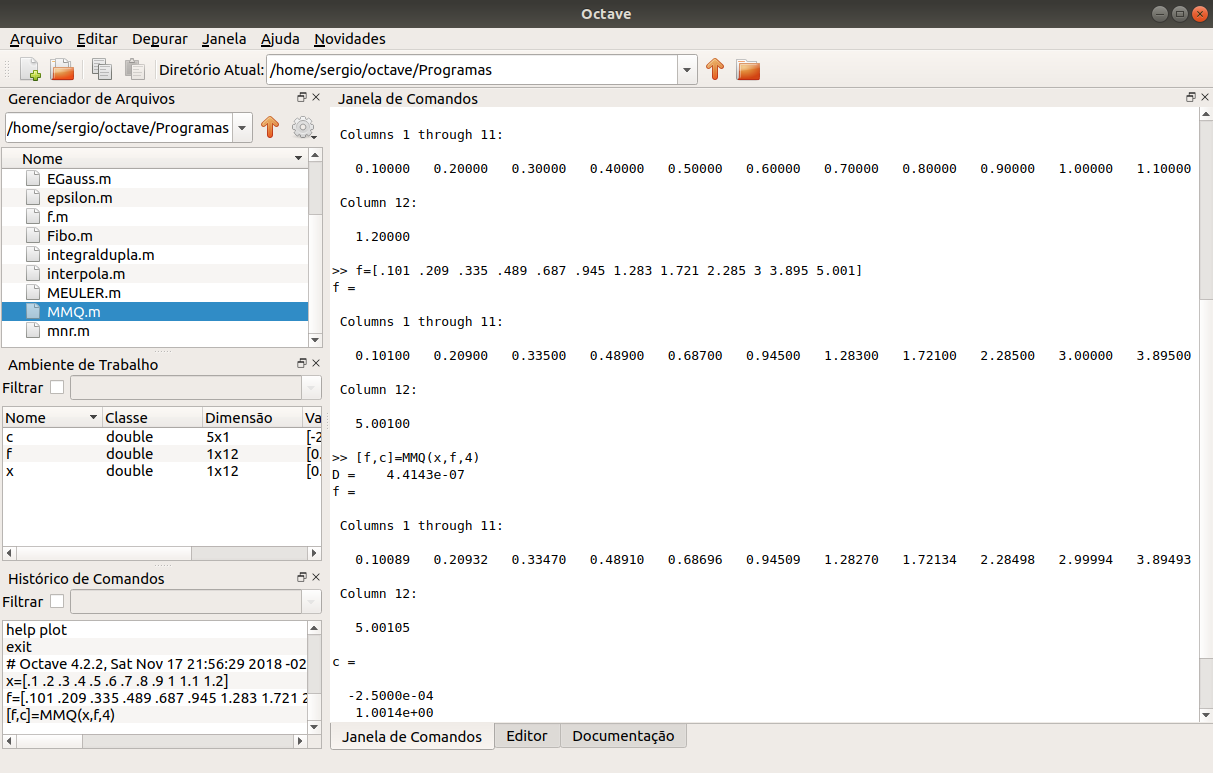
\includegraphics[width=12cm]{octave1.png}
    \caption{Método dos Mínimos Quadrados \label{octave1}}
    
\end{figure}

\begin{figure}[ht]

    \center

    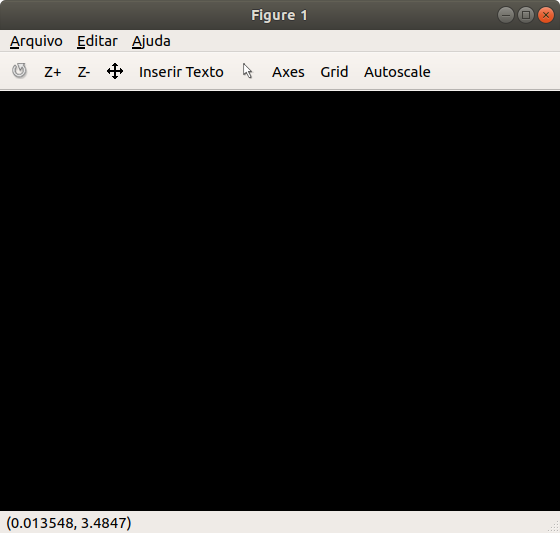
\includegraphics[width=7cm]{grafico1.png}
    \caption{Gráfico MMQ \label{grafico1}}
    
\end{figure}

Nesta figura \ref{grafico1}, estão representados em vermelho os pontos relativos à tabela de dados que inserimos no programa e em azul o gráfico do polinômio encontrado.


\section{Resultados}

Podemos observar pelos resultados e pelo gráfico que, neste caso, a aproximação é excelente, o que nos mostra que esse é um método muito eficiente.


\chapter{Regra de Simpson}



Baseado na Regra de Simpson, vamos determinar uma regra de integração para a integral dupla:

$$\int_a^b\int_c^d f(x,y)\, dx\, dy$$
e aplicá-la para calcular uma aproximação para:
$$I=\int_0^1\int_0^1 x^2 + y^2\, dx\, dy$$

Para resolvermos uma integral dupla, temos que começar de dentro para fora, ou seja, primeiro fixamos $y$ e resolvemos a integral $\displaystyle\int_c^d f(x,y)\, dx$ e posteriormente fixamos x e resolvemos a integral em relação a y. 

Assim teremos: $\displaystyle\int_a^b\int_c^d f(x,y)\, dx\, dy$, chamando a integral $\displaystyle\int_c^d f(x,y)\, dx $ de $G(x)$, podemos escrever:

$$
I=\displaystyle\int_a^b G(x)\, dx
$$


Agora vamos resolver a integral: $I =\displaystyle \int_0^1 \displaystyle\int_0^1 x^2 + y^2\, dx\, dy$ usando a forma acima e o Teorema Fundamental do Cálculo:

$$
\int_0^1 x^2 + y^2\, dx = \left[\frac{x^3}{3} + y^2\cdot x\right]_0^1 =\left[\frac{1^3}{3}+y^2\cdot 1\right]- \left[\frac{0^3}{3}+y^2\cdot 0\right] = \frac{1}{3}+ y^2
$$

Portanto:

$$
I=\int_0^1 \frac{1}{3}+ y^2\, dy = \left[\frac{y}{3} + \frac{y^3}{3}\right]_0^1 =\left[\frac{1}{3} + \frac{1^3}{3}\right]-\left[\frac{0}{3} + \frac{0^3}{3}\right]= \frac{1}{3} + \frac{1}{3} = \frac{2}{3} \cong 0.66666667
$$

\newpage

A partir desse ponto vamos implementar um programa no Octave (usando o Simpson 1/3) que resolva a integral dupla: $I=\displaystyle\int_0^1\displaystyle\int_0^1 x^2 + y^2\, dx\, dy$

A ideia é utilizar a 1ª Regra de Simpson ou regra do 1/3 duas vezes, de tal forma que:

$$ 
I=\displaystyle\int_0^1\displaystyle\int_0^1 x^2 + y^2\, dx\, dy 
$$

Fazendo 
$$
f(x,y)=x^2 + y^2
$$
e
$$
G(y) = \int_{0}^1 f(x,y) dx 
$$
teremos:
$$
I=\int_0^1 G(y) dy
$$
Assim calculamos $G(y_i)$ com $i \in \{0,1,2\}$
$$
G(y_i)= \frac {h} {3} \cdot \left[ f(x_0,y_i) + 4f(x_1,y_i) + f(x_2,y_i) \right]
$$
e, novamente usando a regra de Simpson, temos:
$$
I=\int_0^1 G(y_i) dy = \frac {h} {3} \cdot \left[ G(y_0) + 4G(y_1) + G(y_2) \right]
$$

A programação em \textit{Octave} ficará assim:

\begin{verbatim}
function I=integraldupla(a,b,c,d)
   h1=(b-a)/2;
   h2=(d-c)/2;
   x=[a (a+h1) b];
   y=[c (c+h2) d];
   for i=1:3
      G(i)=(h2/3)*((x(1)^2+y(i)^2)+4*(x(2)^2+y(i)^2)+(x(3)^2+y(i)^2));
   endfor
   I=(h1/3)*(G(1)+4*G(2)+G(3));
endfunction
\end{verbatim}

O programa será chamado indicando os valores de início e fim dos intervalos de integração $a, b, c, d$.

\newpage

O programa após a compilação traz como resultado a figura \ref{octave2}

\begin{figure}[ht]

    \center

    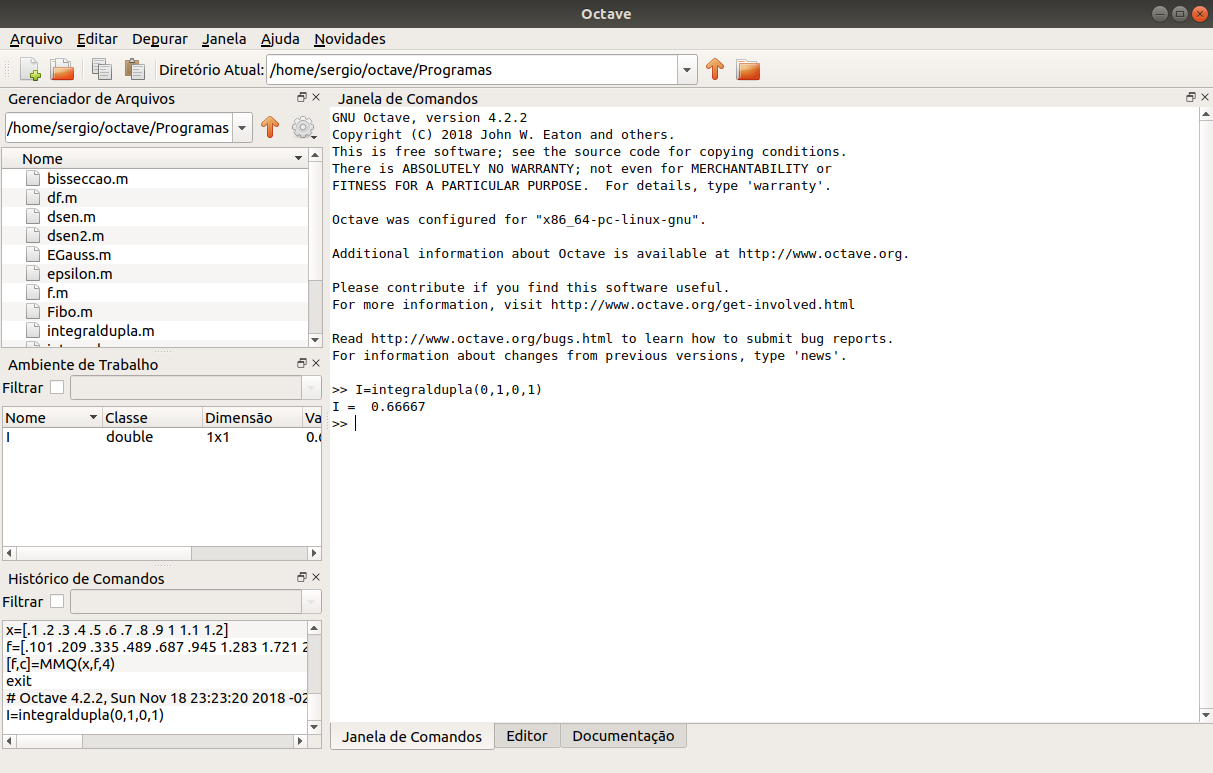
\includegraphics[width=12cm]{octave2.png}
    \caption{Regra de Simpson \label{octave2}}
    
\end{figure}

\section{Resultados}

Apesar de ser uma regra muito simples, podemos perceber olhando a resolução através do Teorema Fundamental do Cálculo e os resultados obtidos por essa regra que é eficiente e que conseguimos um resultado muito próximo.


\chapter{Método de Euler}

Neste projeto vamos fazer um programa para resolver um Problema de Valor Inicial utilizando o Método de Euler.

Vamos encontrar uma aproximação para $y(1.2)$ com $h = 0.1$, para o P.V.I. abaixo:

$$
\left\{\begin{array}{l}
y'' = 3y' - 2y \\ y(0) = -1 \\ y'(0) = 0 
\end{array}\right.
$$

Fazendo: $y'=z$ e $z'=3z - 2y$ resolver esse P.V.I é o mesmo que resolver um sistema do tipo::

$$
\left\{\begin{array}{l}
y'= z \\ z' = 3z-2y \\ y(0) = -1 \\ z'(0) = 0 
\end{array}\right.
$$

Transformando esse sistema em matrizes, temos:

$$
\left[ \begin{array}{c}
y'\\
z'
\end{array} \right] =
\left[\begin{array}{cc}
1 & 0\\
3 & -2
\end{array}\right]\cdot
\left[\begin{array}{c}
z\\
y
\end{array}\right]
$$

Assim fazemos

$$
f\left(\left[ \begin{array}{c}
y\\
z
\end{array} \right]\right) =
\left[\begin{array}{cc}
1 & 0\\
3 & -2
\end{array}\right]\cdot
\left[\begin{array}{c}
z\\
y
\end{array}\right]
$$

E pelo Método de Euler, usaremos a seguinte recorrência para resolvê-la:

$$
\left[
\begin{array}{c}
y_{k+1}\\
z_{k+1}

\end{array}\right] =
\left[
\begin{array}{c}
y_{k}\\
z_{k}
\end{array}\right] + h\cdot
f\left(\left[
\begin{array}{c}
y_{k}\\
z_{k}
\end{array}\right]\right)
$$

\newpage

Implementando um programa \textit{Octave} para resolvê - la, temos:

\begin{verbatim}
function y=MEULER(h,x,y0,z0)
  t=ceil(x/h);
  Yn=[y0;z0];
  S=[1 0;3 -2];
  Ya=[Yn(2,1);Yn(1,1)];
  f=S*Ya;
  for i=1:t+1
      Yn=Yn+h*f;
     Ya=[Yn(2,1);Yn(1,1)];
    f=S*Ya;
  endfor
  y=Yn(1);
endfunction
\end{verbatim}

Neste programa indicamos o valor de $h$, de $x$ para a aproximação, de $y(0)$ e de $z(0)$ e resultado podemos ver através da figura \ref{octave3}

\begin{figure}[ht]

    \center

    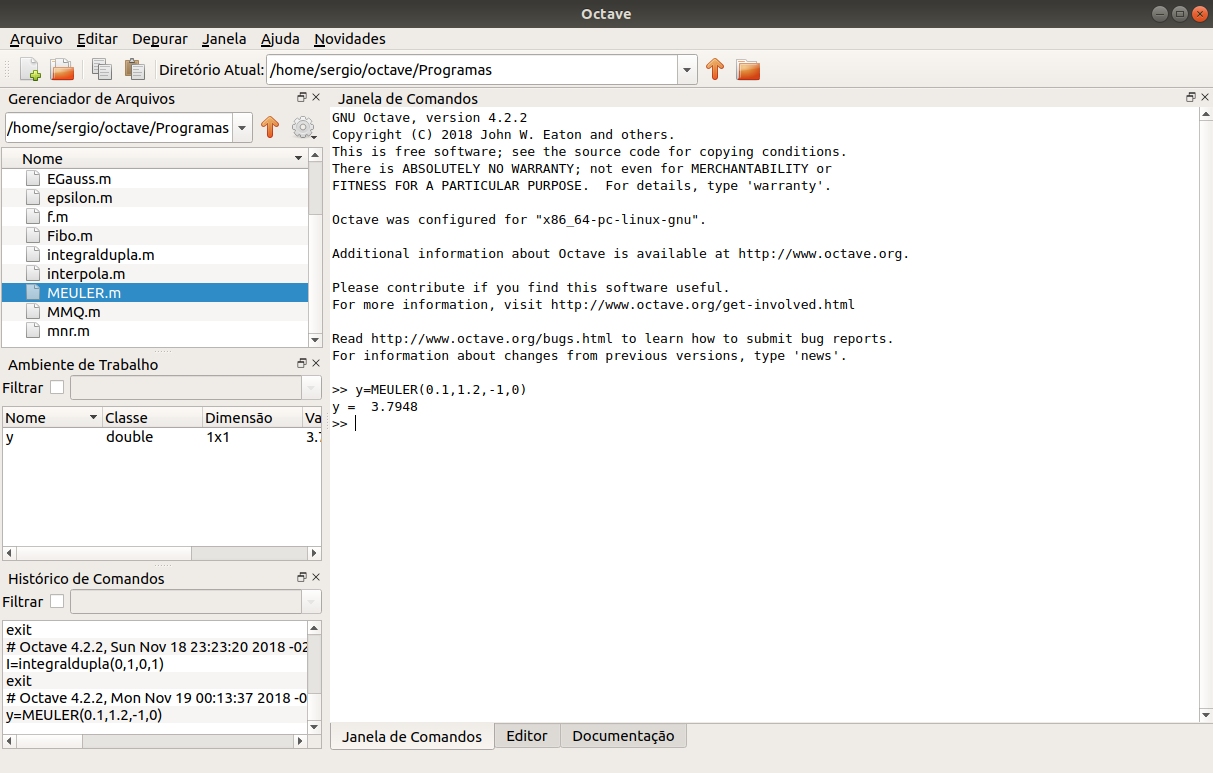
\includegraphics[width=12cm]{octave3.png}
    \caption{Método de Euler \label{octave3}}
    
\end{figure}

\section{Resultado}

Com um pouco de trabalho algébrico é possível resolver a equação diferencial de 2ª ordem, ou seja: $y'' = 3y' - 2y \Rightarrow y=c_1e^{2x} + c_2e^{x}$. Substituindo $y(0) = -1$ e $y'(0) = 0$, encontraremos: 
$$y=e^{2x} - 2\cdot e^{x}$$

Calculando $y(1,2)$ na função acima encontraremos o valor: $y(1,2) = 4,3829$ que representa o valor real. Essa diferença se dá porque quando escolhemos $h = 0,1$ no \textit{Octave}, tivemos que dividir o intervalo entre o valor inicial e o valor final de $x$ em 12 partes e por isso o erro. Usando o mesmo programa, mas diminuindo o valor de $h$ no octave conseguimos uma aproximação mais próxima do valor real de $y(1,2)$.

Vamos colocar outros valores para o $h$, simulando para $h = 0.01$ e $h = 0.001$ e podemos ver o resultado através da figura \ref{octave4}:

\begin{figure}[ht]

    \center

    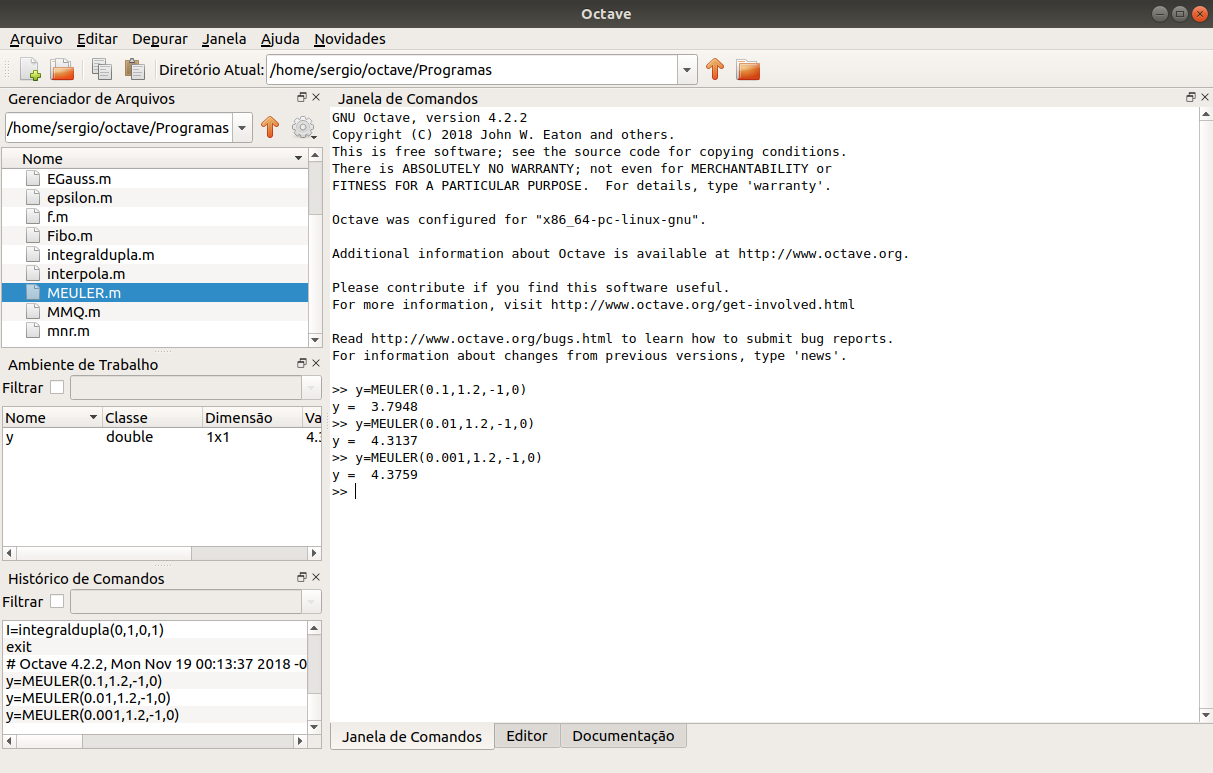
\includegraphics[width=11cm]{octave4.png}
    \caption{Método de Euler com $h$ modificado\label{octave4}}
    
\end{figure}

Este resultado é muito mais próximo do real. Podemos perceber então que o resultado depende muito do valor de $h$ e que o erro pode ser diminuido se o intervalo for menor e o valor de $h$ também.



\end{document}
